\section{Exploring The Z-Profile}
\label{ch:ExploringZProfile}

\begin{frame}{New Bunch Alignment}
\begin{figure}
\begin{center}
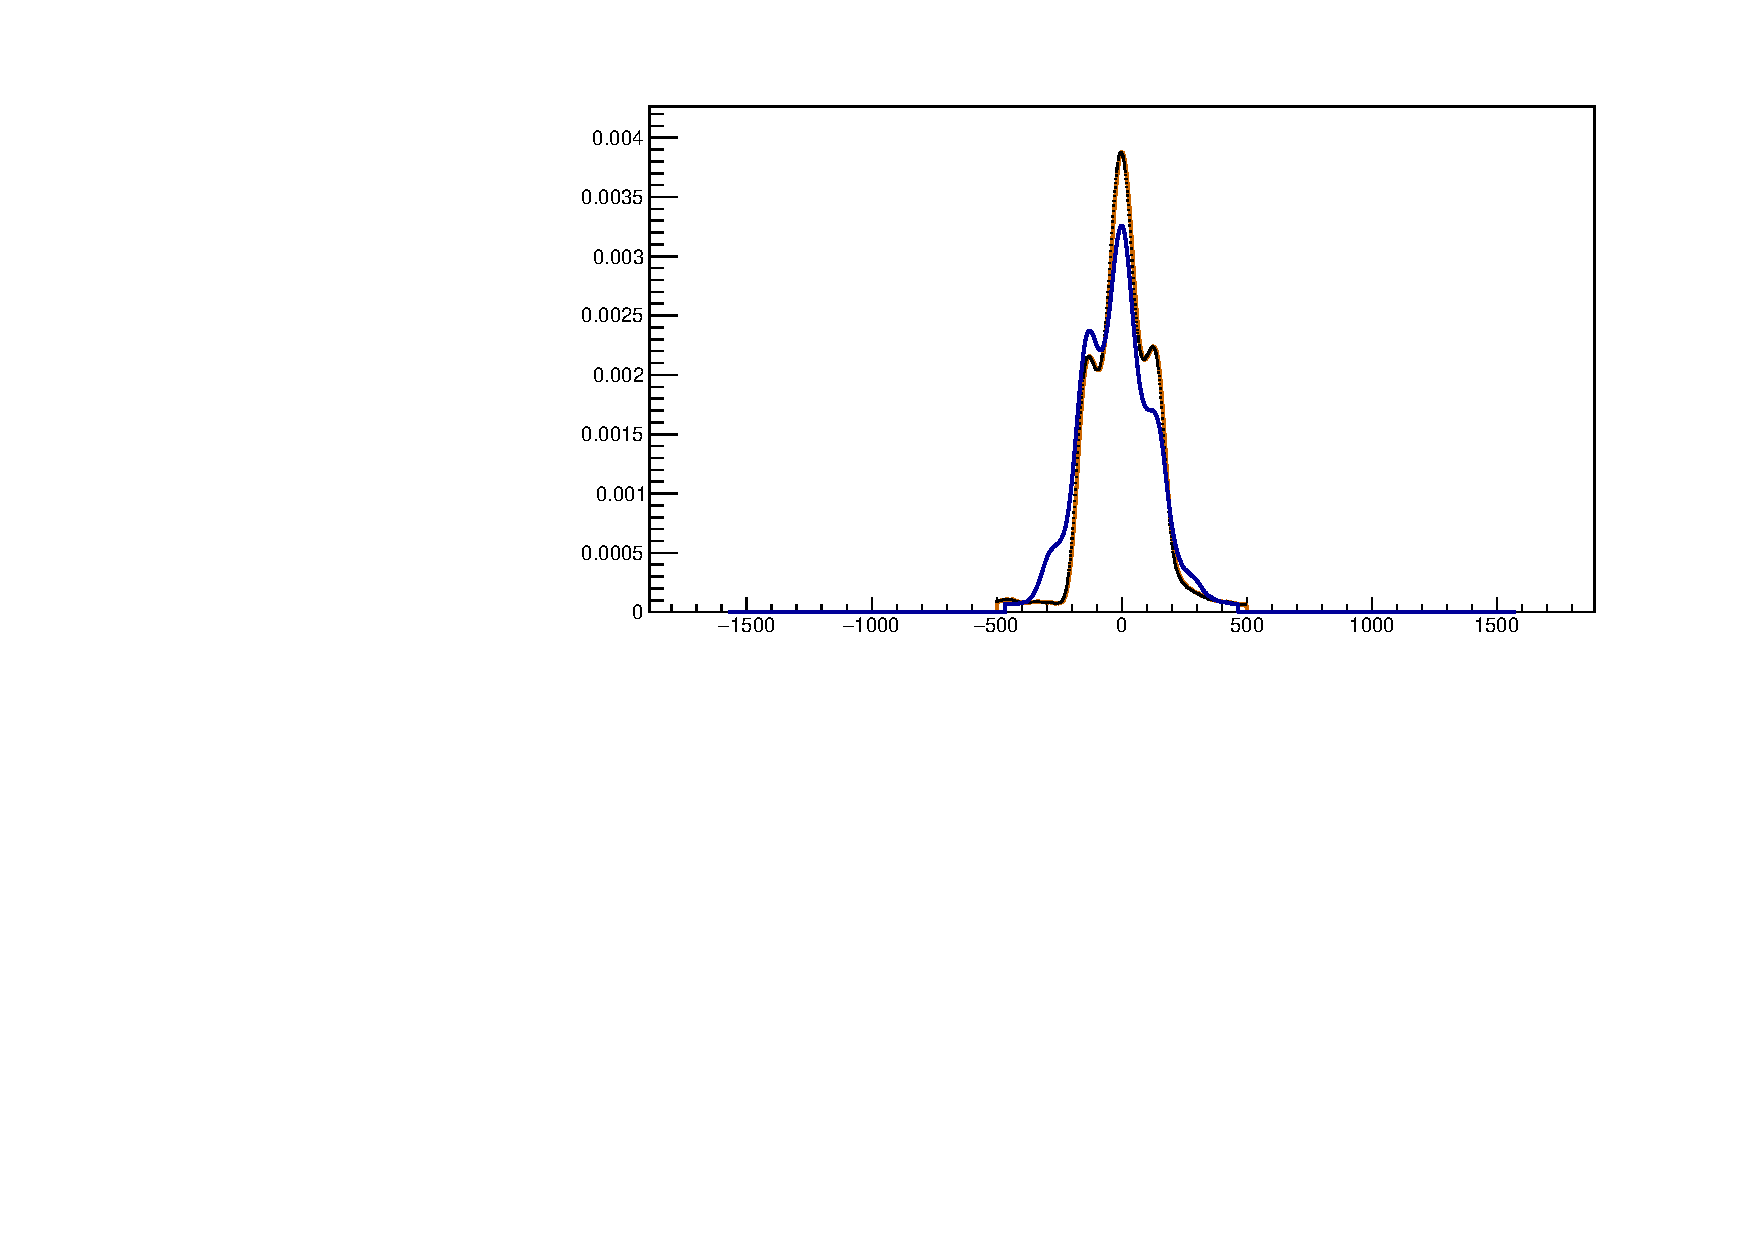
\includegraphics[width=0.8\linewidth]{../ExploringZProfile/figs/359711_bunch_alignment.pdf}
\end{center}
\caption{Bunches have been aligned such that they line up at their maxima,
rather than lining up according to a time window. We define the time binning such
that at arbitrary time t = 0, these maxima overlap.}
\label{fig:359711_bunch_alignment}
\end{figure}
\end{frame}

\begin{frame}{Lookup Accuracy}
\begin{figure}
\begin{center}
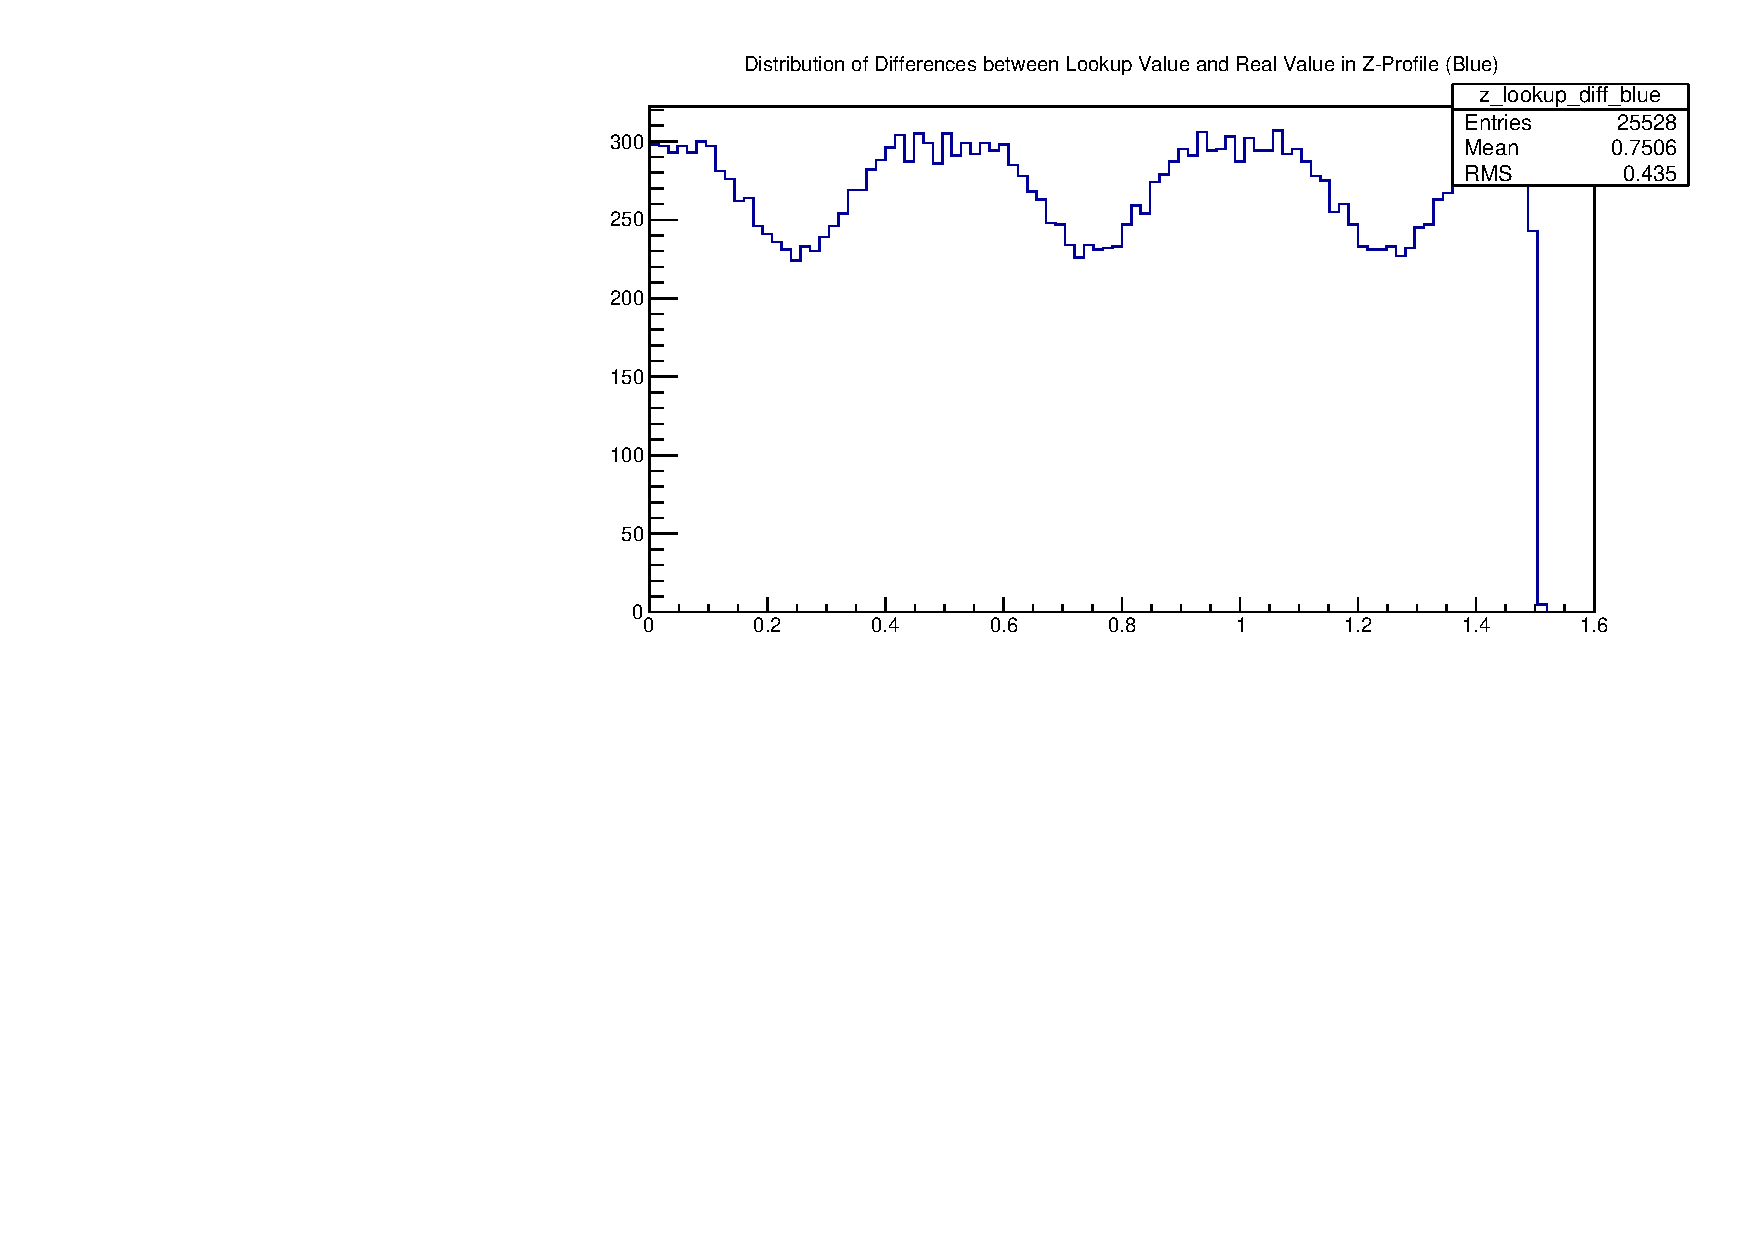
\includegraphics[width=0.8\linewidth]{../ExploringZProfile/figs/359711_lookup_z.pdf}
\end{center}
\caption{Instead of interpolation between defined profile points, we instead bin
time finely, which results in a spatial binning of 1.5 cm in z. Pictured here
is a histogram, binned in z, where we fill it with the difference between the
looked up z value, and the z-value desired. The yellow beam lookup calls are
identical.}
\label{fig:359711_lookup_z}
\end{figure}
\end{frame}

\begin{frame}{Do Bunches Collide Maximally Overlapped?}
\begin{figure}
\begin{center}
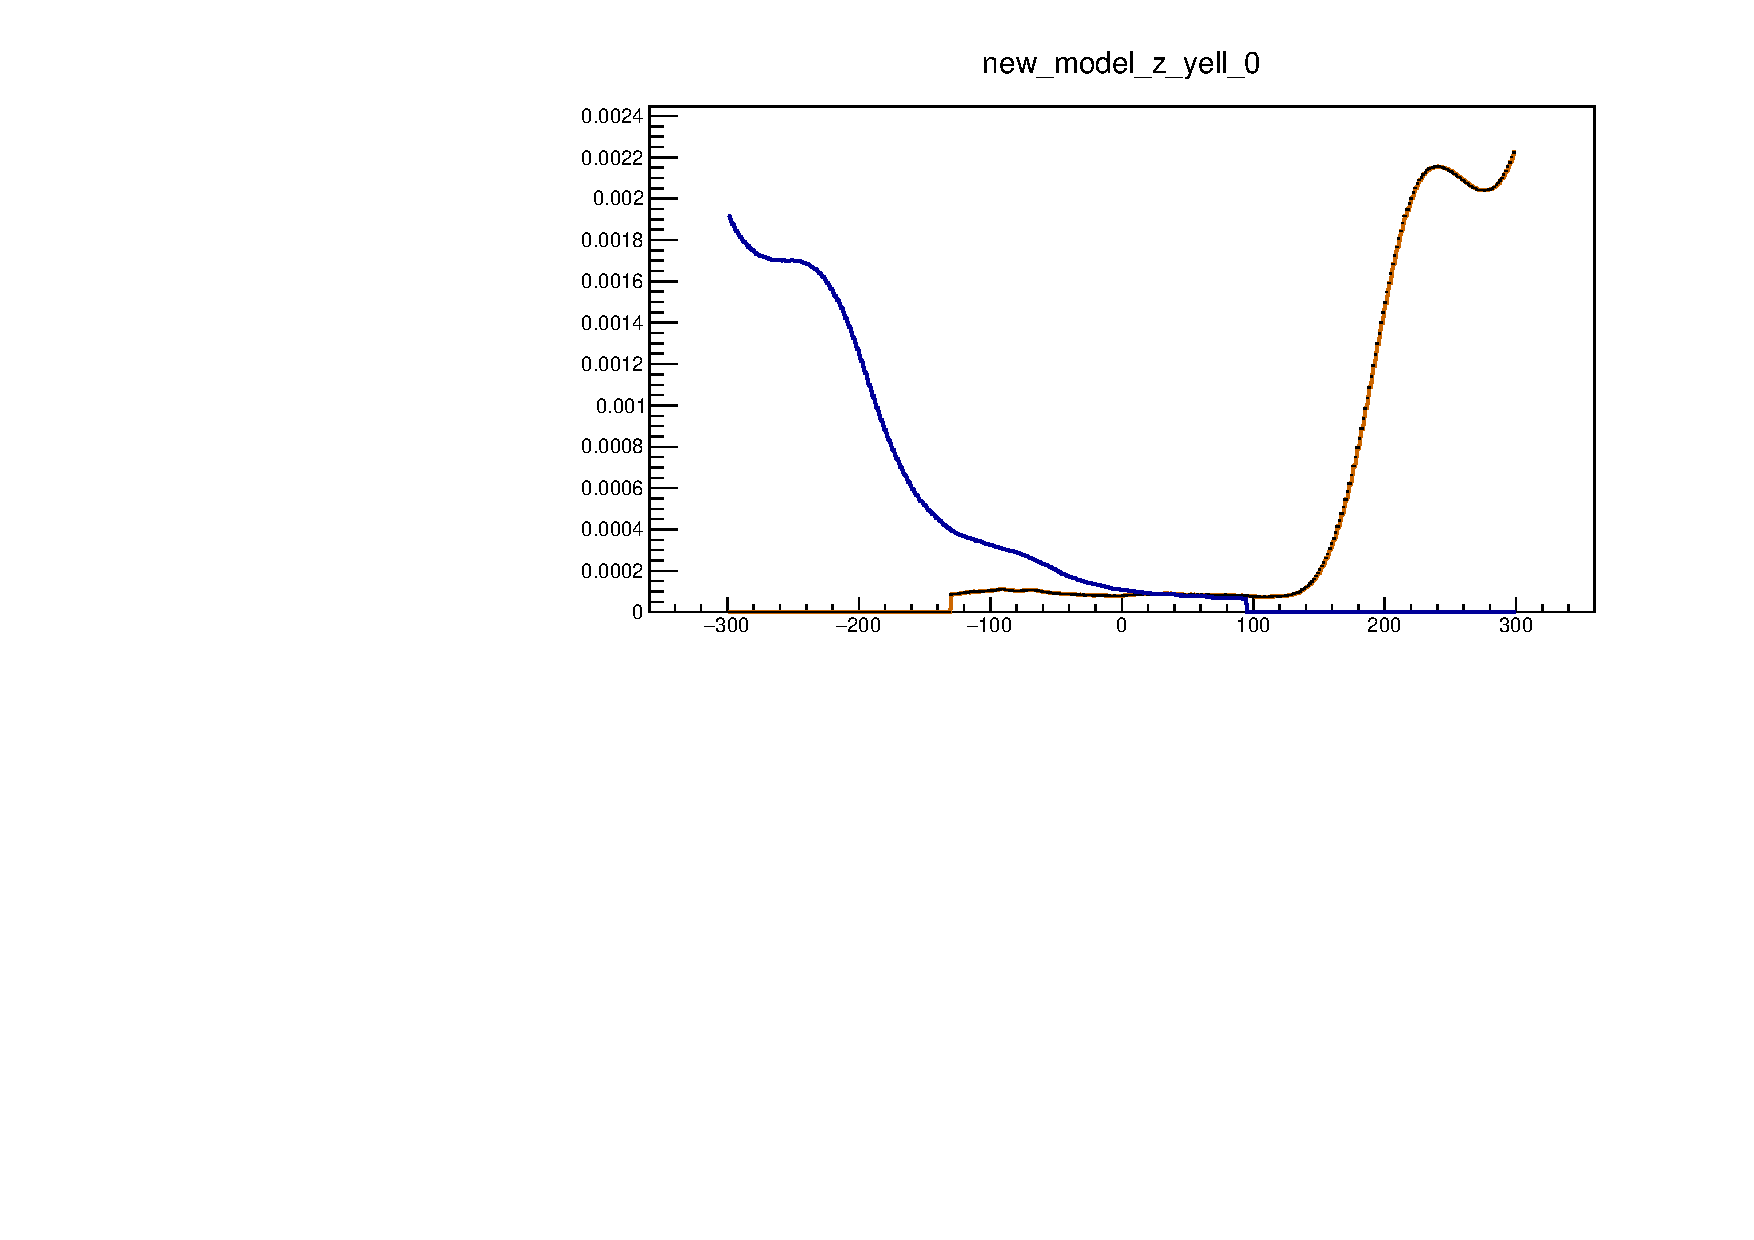
\includegraphics[width=0.8\linewidth]{../ExploringZProfile/figs/359711_time_step_0_bunch_collision.pdf}
\end{center}
\caption{Pictured here, we observe the blue and yellow bunches from a fixed
point in space (z = 0). Blue is incoming from the right, yellow, from the left.
The time resolution of the simulation is $\approx$2.5 ns. Shown: 12.5 ns before
collision }
\label{fig:359711_time_step_0_bunch_collision}
\end{figure}
\end{frame}

\begin{frame}{Do Bunches Collide Maximally Overlapped?}
\begin{figure}
\begin{center}
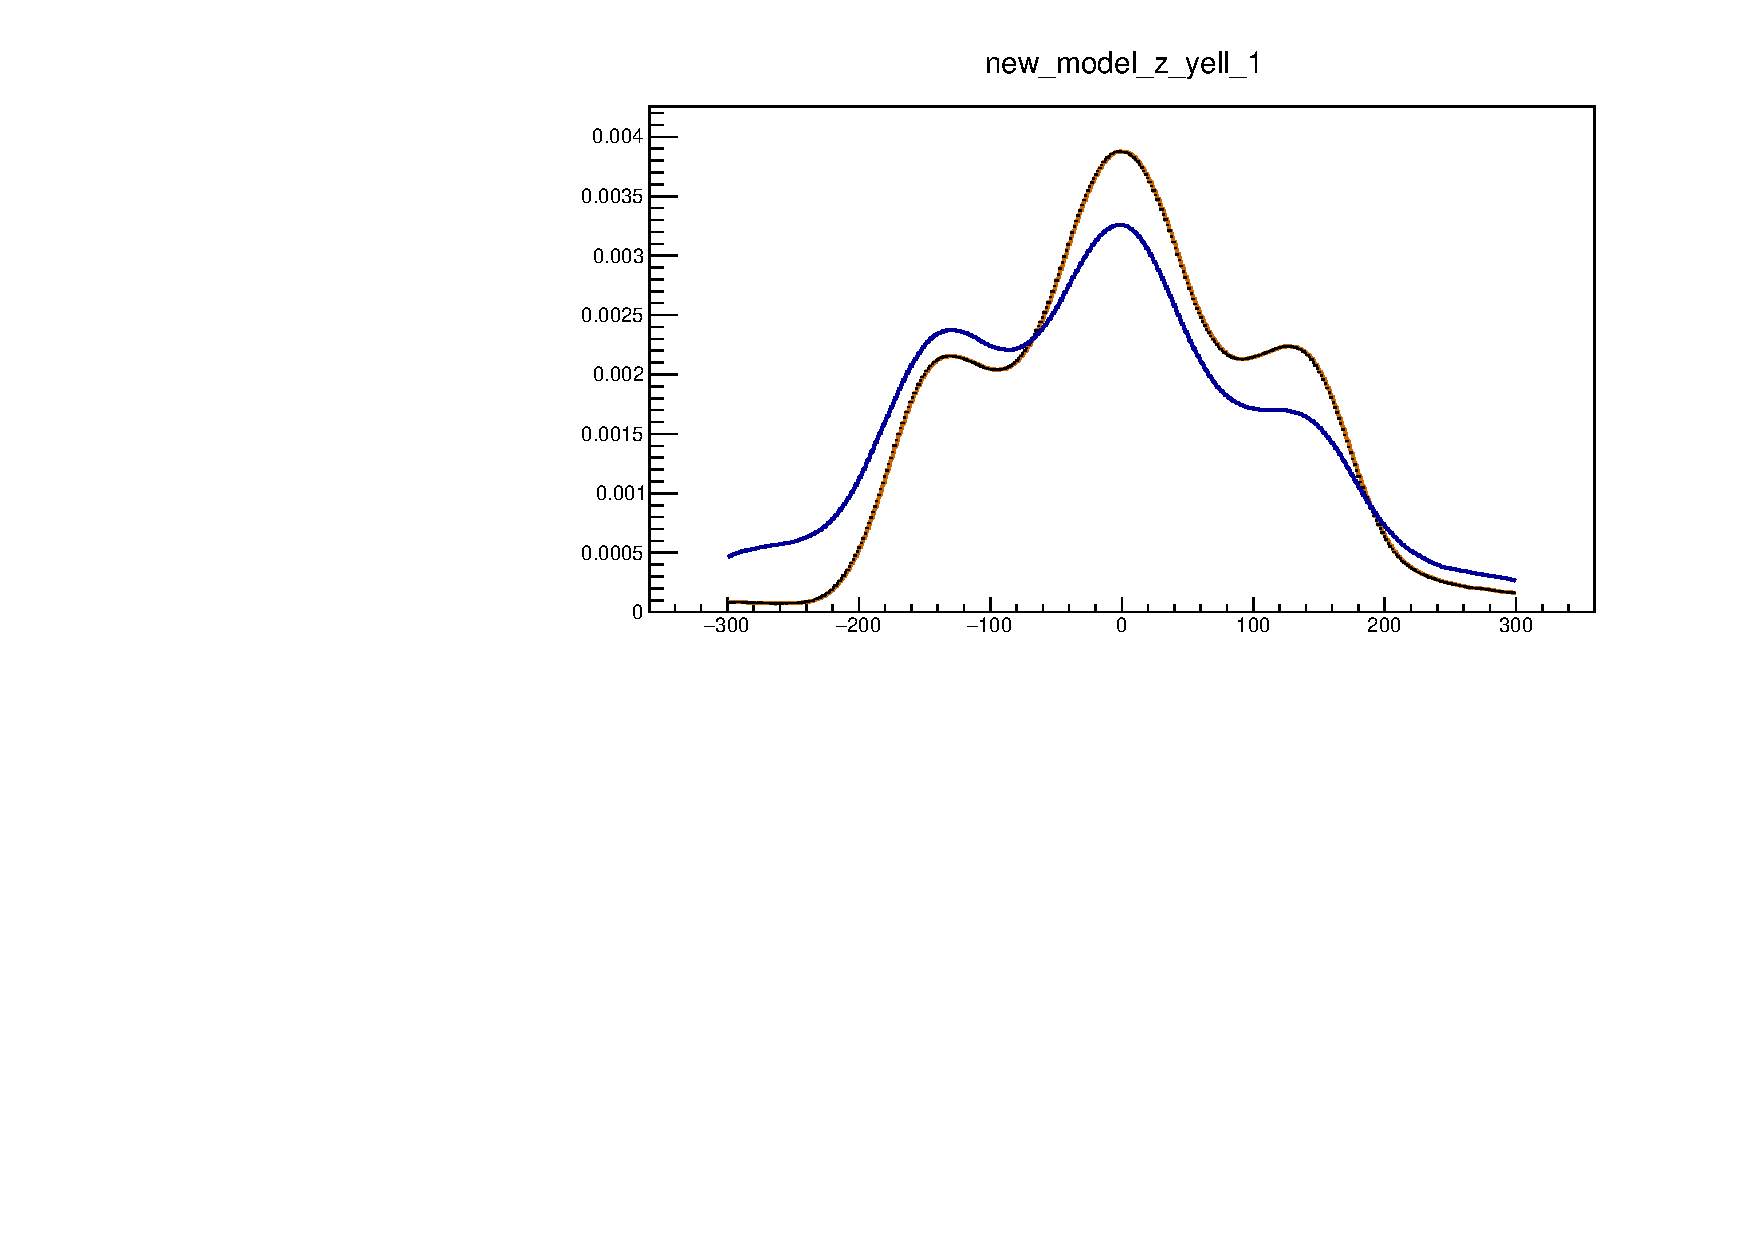
\includegraphics[width=0.8\linewidth]{../ExploringZProfile/figs/359711_time_step_1_bunch_collision.pdf}
\end{center}
\caption{Pictured here, we see the blue and yellow bunches at the nominal
interaction time, t = 0. The maxima of each bunch aligns exactly with z = 0.
Again, we observe from a fixed point in space, at z = 0. }
\label{fig:359711_time_step_1_bunch_collision}
\end{figure}
\end{frame}

\begin{frame}{Do Bunches Collide Maximally Overlapped?}
\begin{figure}
\begin{center}
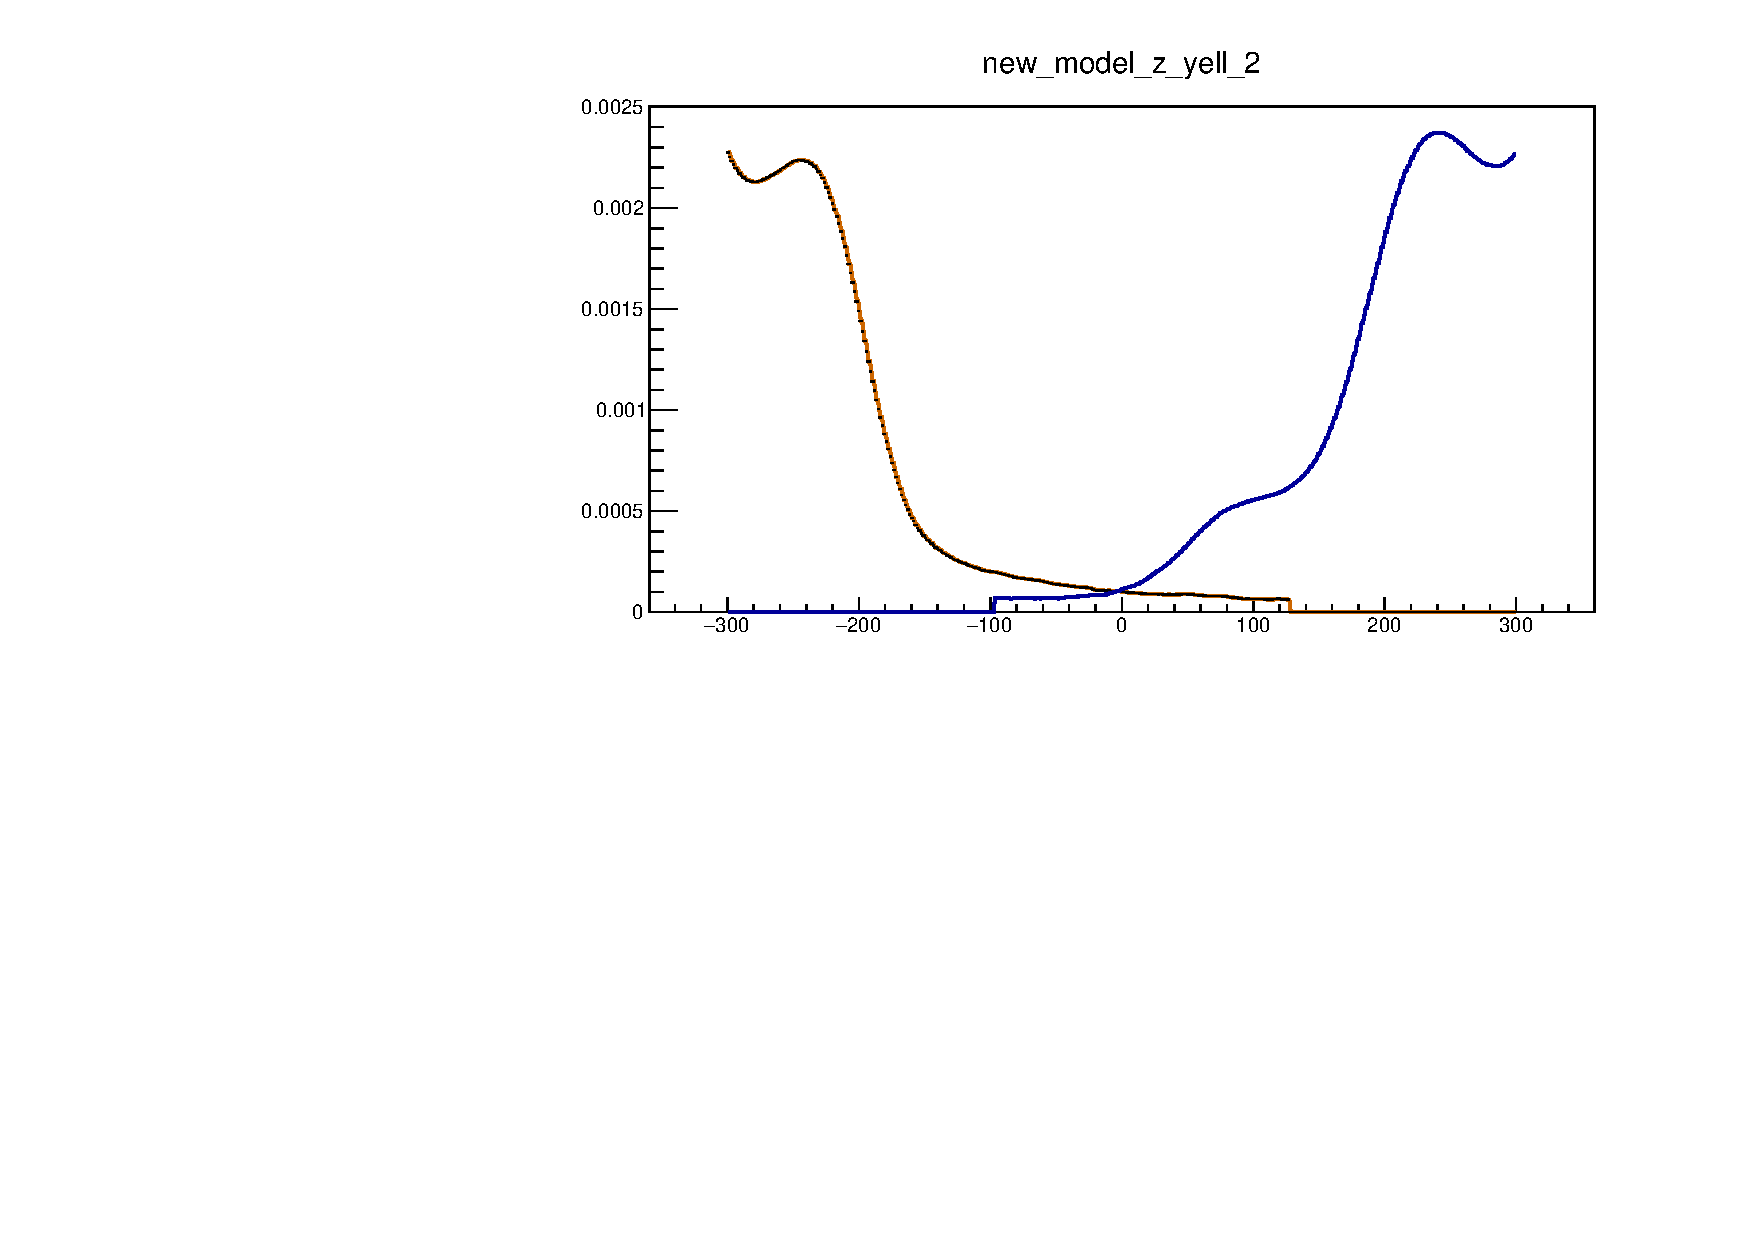
\includegraphics[width=0.8\linewidth]{../ExploringZProfile/figs/359711_time_step_2_bunch_collision.pdf}
\end{center}
\caption{Finally, we observe the bunches after the nominal interaction time,
from a fixed z-position. Another 12.5 ns have passed, and we can see the blue
bunch as continued to the right, and the yellow to the left.}
\label{fig:359711_time_step_2_bunch_collision}
\end{figure}
\end{frame}

\begin{frame}{Resulting ZDC Z-Profile}
\begin{figure}
\begin{center}
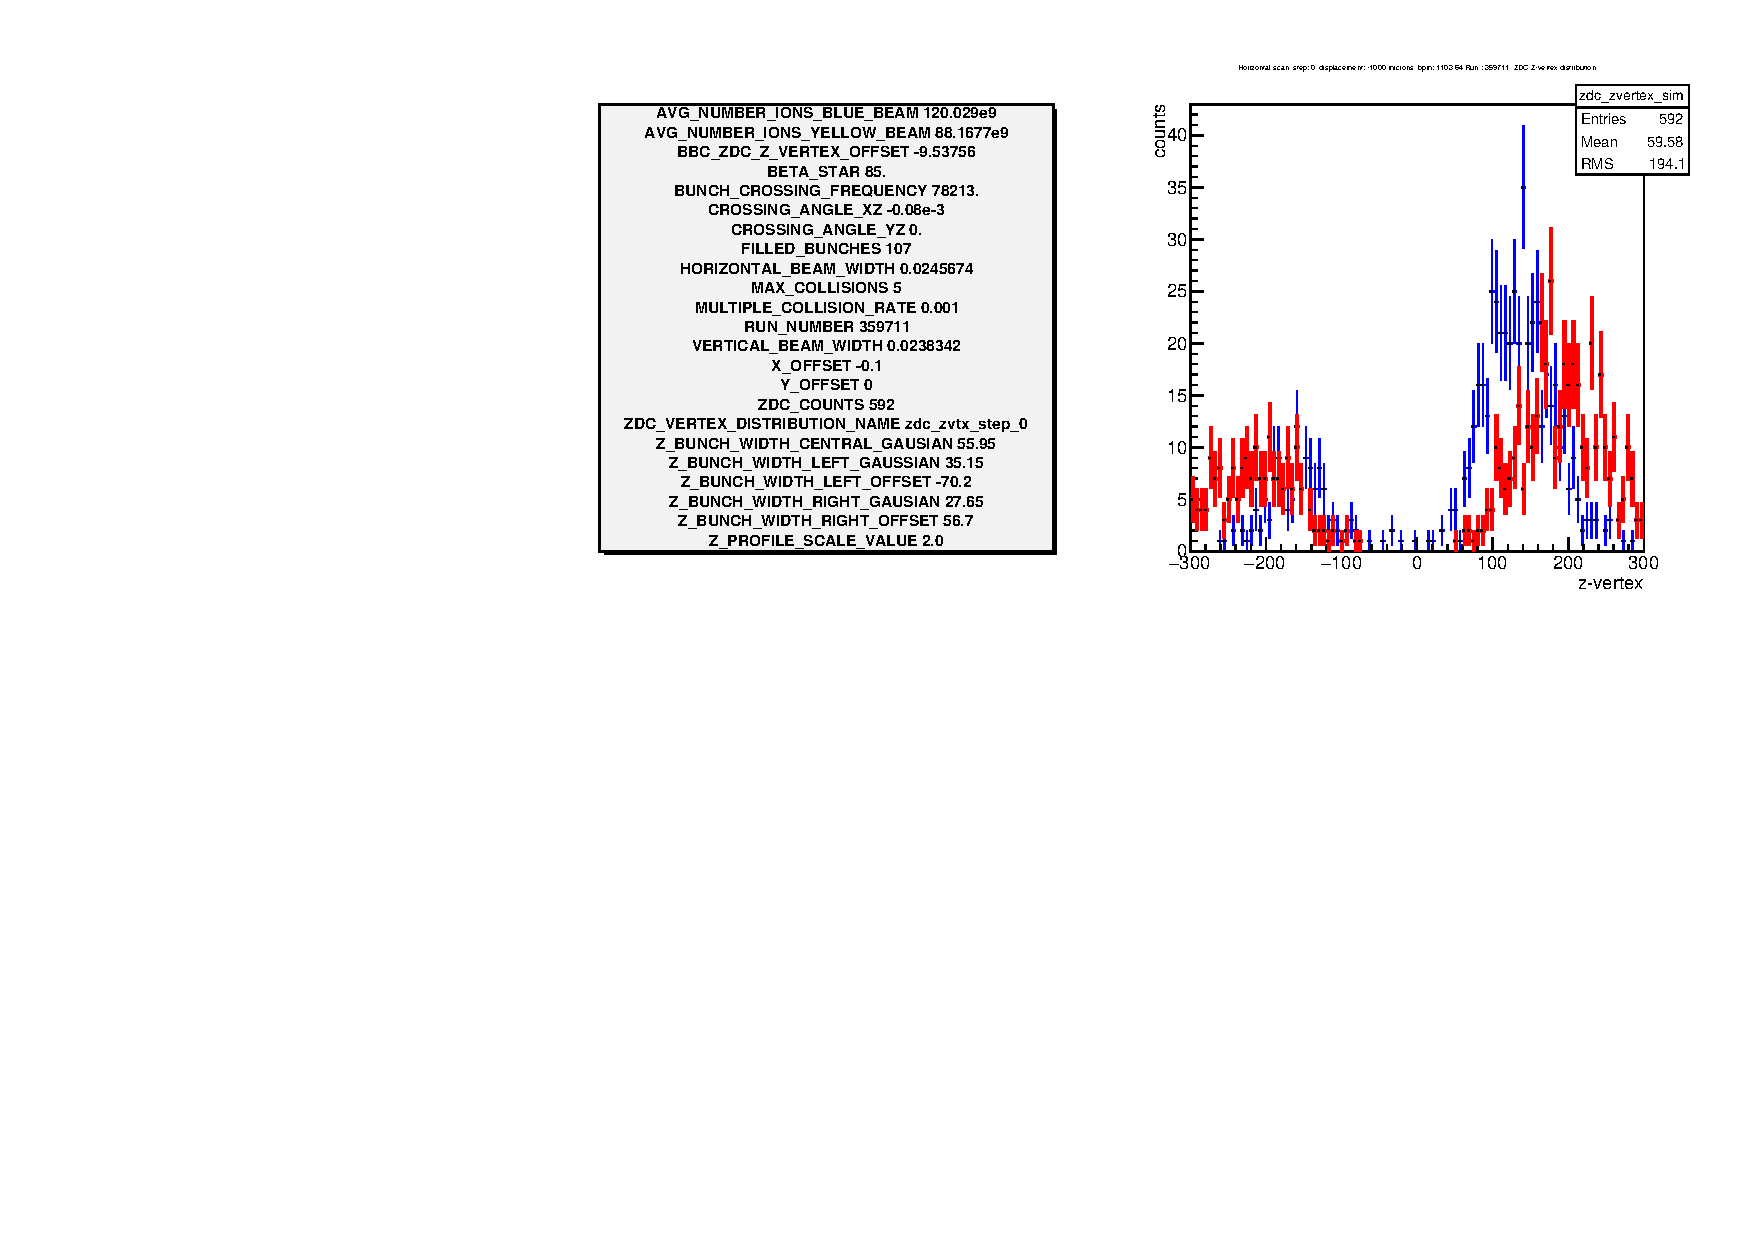
\includegraphics[width=0.8\linewidth]{../ExploringZProfile/figs/359711_step_0_zvertex_compare.pdf}
\end{center}
\caption{We get slightly better results by adjusting the interaction between
bunches to overlap at z = 0, but the distribution is still not well aligned. The
peaks seem to be separated too much.}
\label{fig:359711_step_0_zvertex_compare}
\end{figure}
\end{frame}

\begin{frame}{Resulting ZDC Z-Profile - With Hand Tuning}
\begin{figure}
\begin{center}
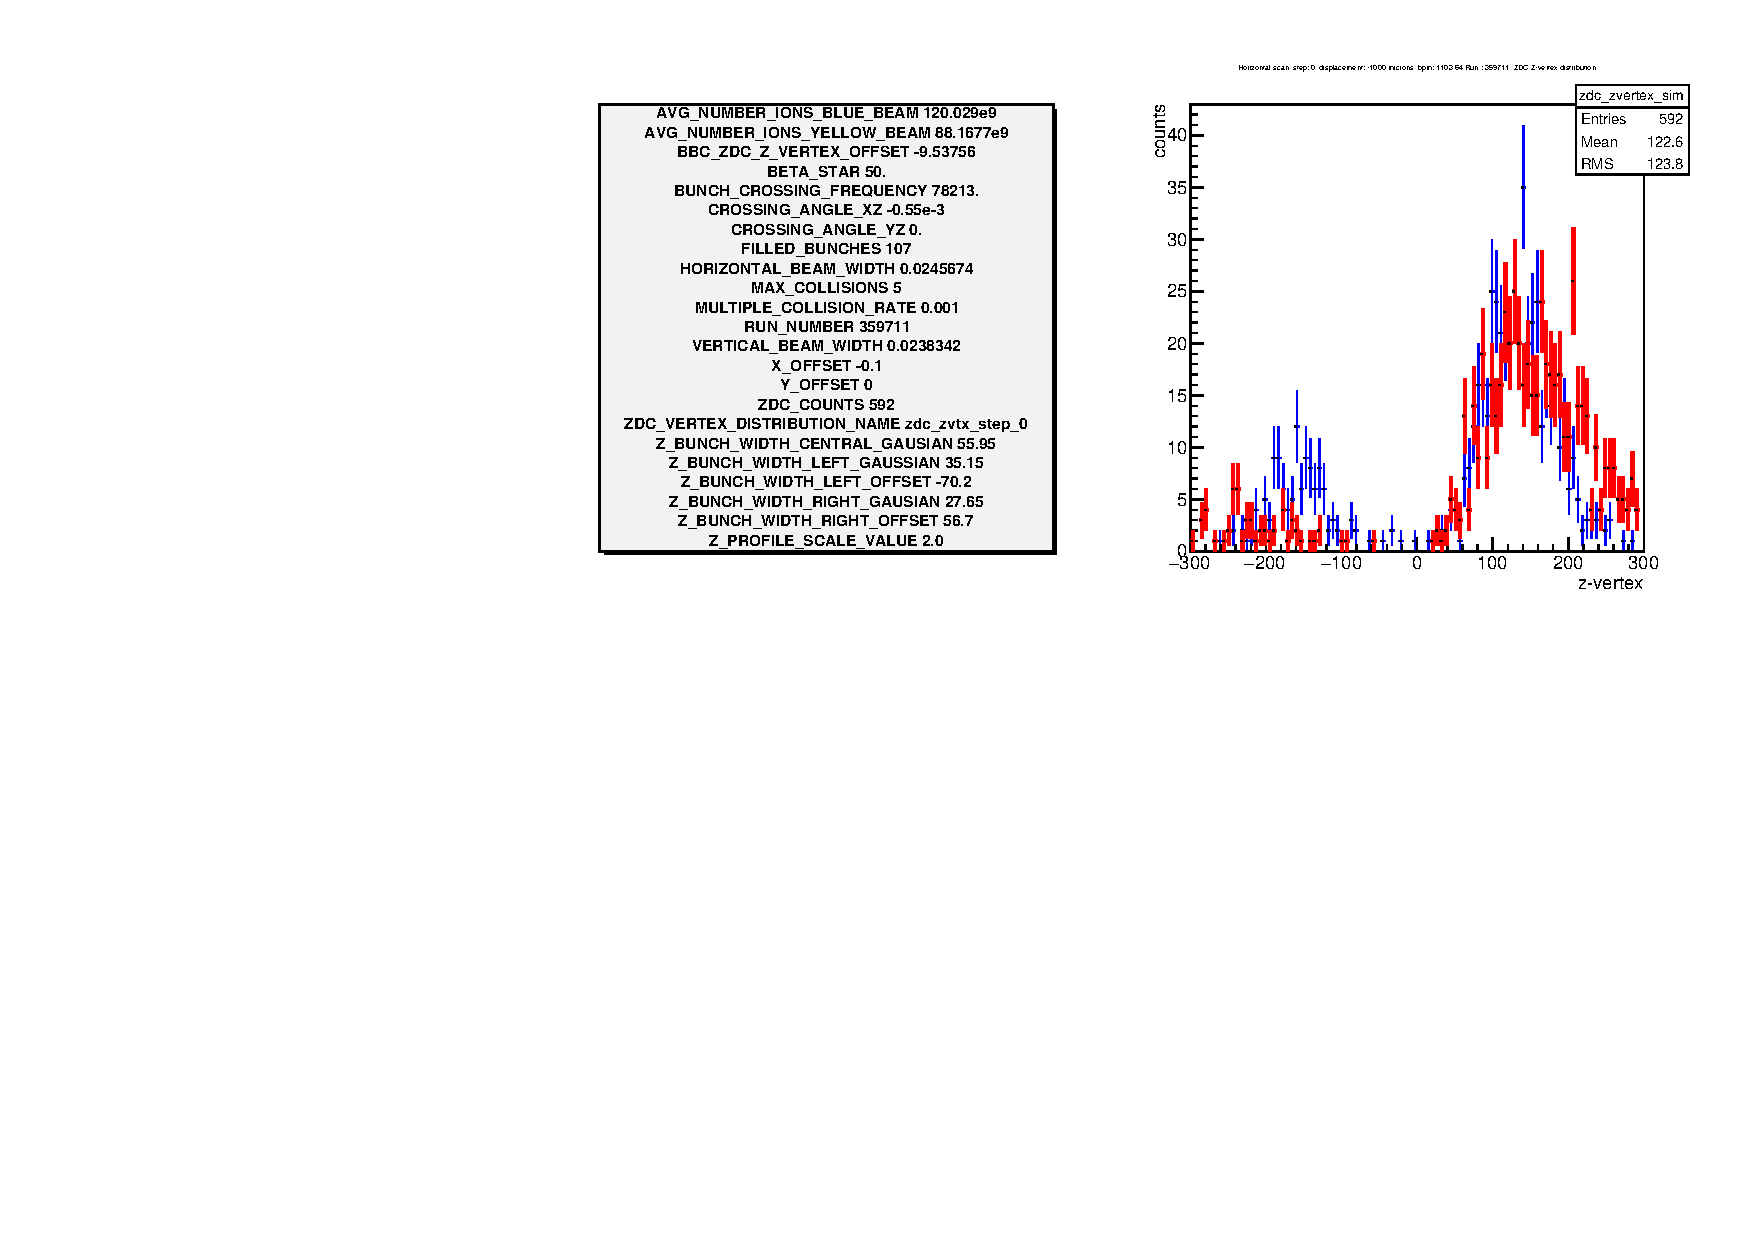
\includegraphics[width=0.8\linewidth]{../ExploringZProfile/figs/359711_step_0_zvertex_compare_tuned.pdf}
\end{center}
\caption{We get slightly better results by tuning $\theta_{XZ}$ and $\beta^{*}$.
	As expressed in previous weeks, I am concerned that the simulations present a
	fine tuning problem. The distributions seem to exhibit the right sort of
behavior at maximum and minimum overlap.}
\label{fig:359711_step_0_zvertex_compare_tuned}
\end{figure}
\end{frame}

\begin{frame}{Resulting ZDC Z-Profile - With Hand Tuning}
\begin{figure}
\begin{center}
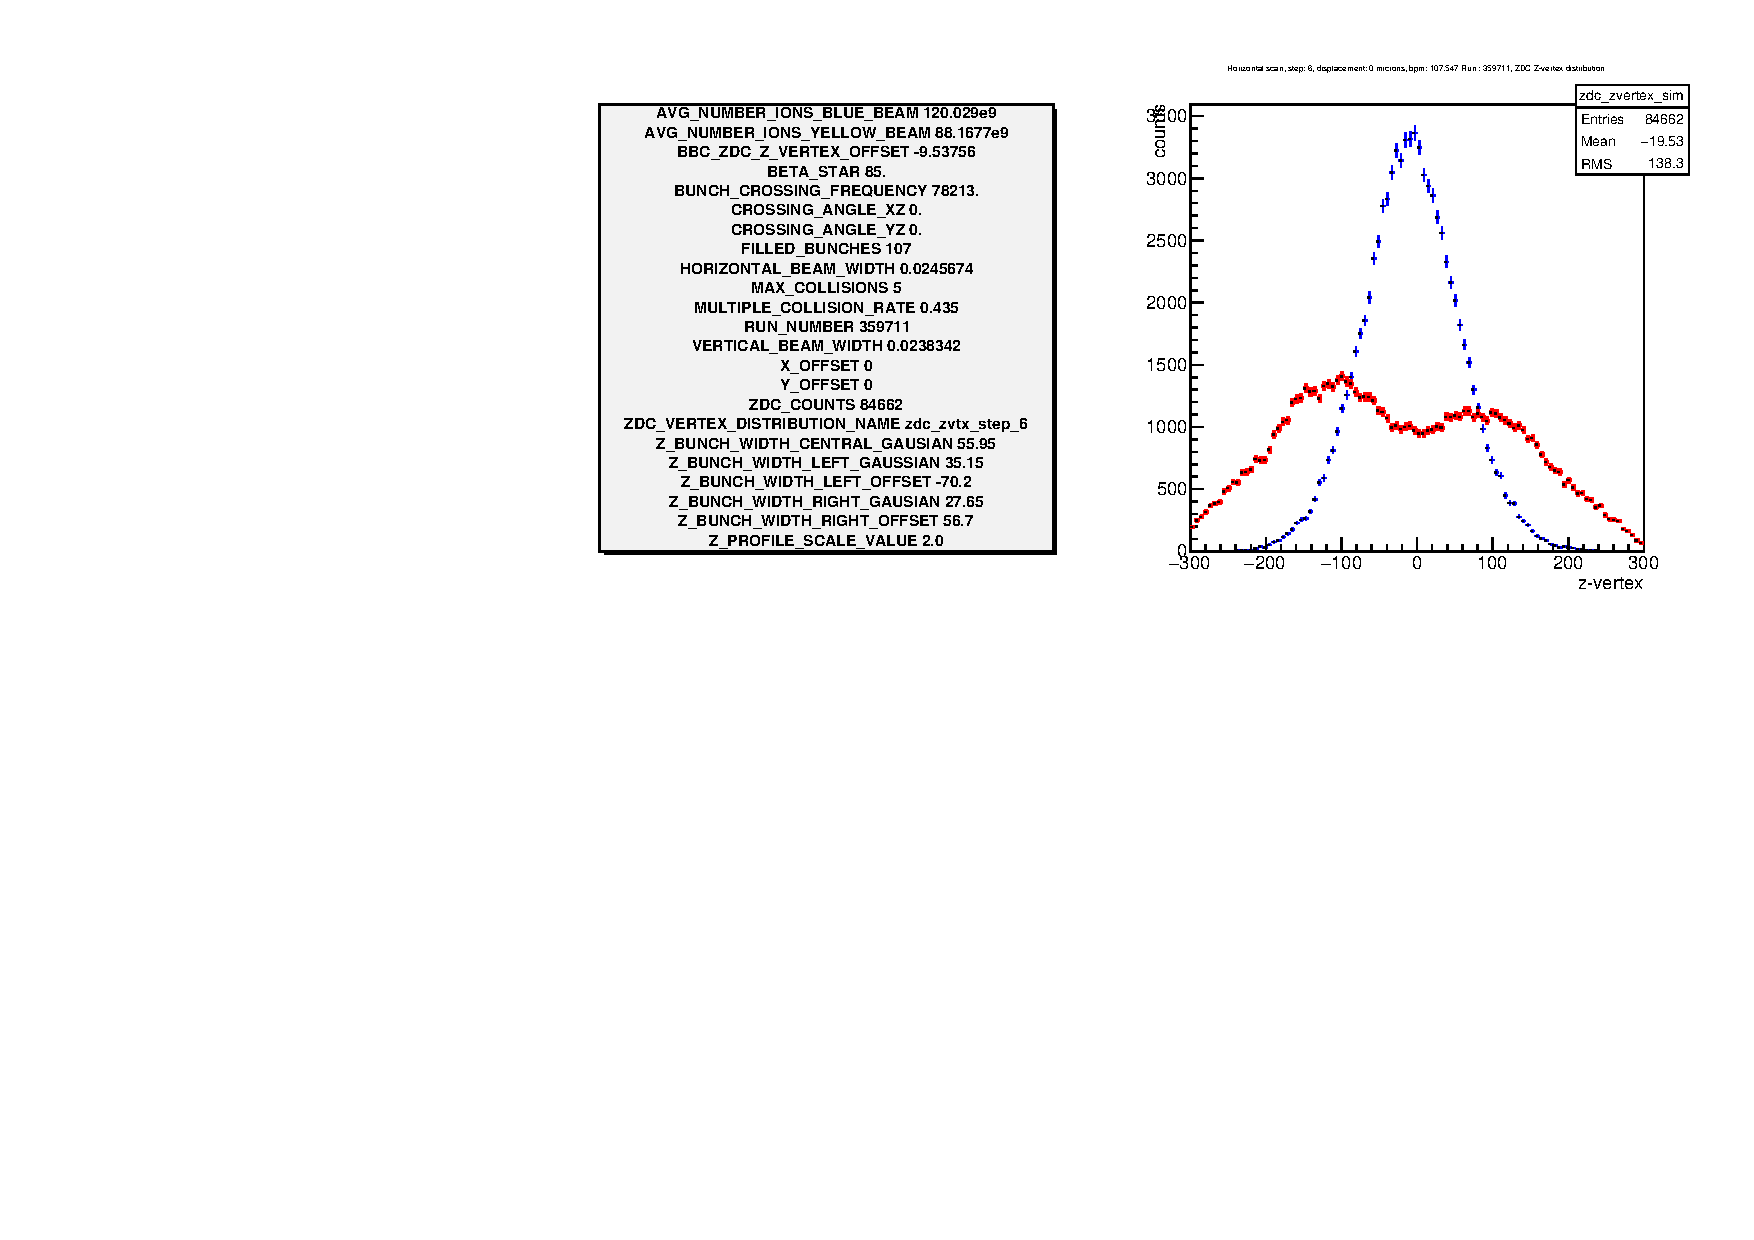
\includegraphics[width=0.8\linewidth]{../ExploringZProfile/figs/359711_step_6_zvertex_compare.pdf}
\end{center}
\caption{As a sanity check for the WCM z-profile driven simulation, as Sasha
	recommended last week, we look at the maximum overlap distribution. The
	simulated beams do not seem to be aligned, though there is no offset provided
	in the horizontal or vertical directions. I'm not sure what is causing this
behavior}
\label{fig:359711_step_6_zvertex_compare}
\end{figure}
\end{frame}


\begin{frame}{Discussion}
	\begin{itemize}
		\item So far, we are not getting good results from the WCM z-profiles.
		\item What else could be causing this behavior...(assumption is bug in code,
			but where)
		\item Lets assume that the z-profiles are okay, and move on to other tuning
			methods.
		\item But first, lets directly compare the simple z-profile to the
			realistic z-profile.
	\end{itemize}
\end{frame}
